% this file is called up by thesis.tex
% content in this file will be fed into the main document

\ifpdf
\graphicspath{{4_konzept/figures/PNG/}{4_konzept/figures/PDF/}{4_konzept/figures/}}
\else
    \graphicspath{{4_konzept/figures/EPS/}{4_konzept/figures/}}
\fi

%: ----------------------- introduction file header -----------------------
\chapter{Konzeptionelle Ueberlegungen}
\label{chapter:konzeptionelle_ueberlegungen}
Die vorangegangenen Auseinandersetzungen mit den Themen COPD und Musiktherapeutische Stimmarbeit dienten dem Aufbau einer Basis, um nun auf dieser ein eigenes Konzept entwickeln zu können. 

Dieses Konzept für die musiktherapeutische Stimmarbeit mit COPD-Patienten ist als übungs- und erlebniszentriertes sowie ressourcenorientiertes Gruppenverfahren angelegt, welches auf der Grundlage psychodynamisch orientierter Musiktherapie Aspekte aus der Körper- und Atemarbeit, Achtsamkeitslenkung und Gesangspädagogik mit einbezieht. Die folgenden Abschnitte sollen dies nun weiter ausführen und erklären. Am Ende des Kapitels wird ein beispielhafter Sitzungsaufbau beschrieben. Um für die Praxis gut vorbereitet zu sein, wurden im Verlauf des Masterarbeits-Prozesses verschiedene Übungen gesammelt, welche jedoch aus Platzgründen zum Teil dem Anhang zum interessierten Nachlesen beigefügt wurden.


\section{Psychodynamische Überlegungen}
\label{psychodynamische ueberlegungen}
In \ref{copd} wurde bereits dargelegt, dass die Diagnose einer COPD auch auf psychischer Ebene für Patienten mit Veränderungen verbunden sein kann. In welchem Ausmaß dies geschieht und mit welchen Folgen es verbunden sein kann, ist sehr individuell verschieden und hängt mit den jeweiligen biographischen Hintergründen und den damit verbundenen Entwicklungsmöglichkeiten hinsichtlich einer stabilen, gefestigten psychischen Verfassung sowie mit einem unterstützenden sozialen Umfeld zusammen. 
Wie bereits unter 2. näher erläutert, wird eine COPD nur unter bestimmten Umständen ausgebildet: genetische Veranlagung (ein sehr verschwindend geringer Teil), Umweltverschmutzung und Einatmen von Schadstoffen bspw. im beruflichen Umfeld sowie zum größten Teil durch einen länger andauernden Nikotin-Abusus (betrifft ca. 80\% der Patienten). 

Was bedeutet aber letzteres nun für die therapeutische Behandlung dieser Patienten? M.E. scheint es wichtig diesen Aspekt mitzudenken und aufzugreifen, da damit oftmals  suchtspezifische psychische Aspekte verbunden sind und diese Besonderheiten insbesondere in der Gegenübertragung mit sich bringen und somit für die Behandlung abhängiger Patienten die Auseinandersetzung mit diesem Thema seitens des Therapeuten unumgänglich erscheint. Es ist mir natürlich bewusst, dass mit dieser Erklärung nicht alle potentiellen Patienten eingeschlossen sein werden, aber aufgrund der hohen Relevanz der Nikotinabhängigkeit in Verbindung mit der Ausbildung einer COPD bedarf es eines Einbezugs dieser Problematik in therapeutische Konzepte. Es gilt natürlich in der Praxis diese Annahmen stets zu überprüfen und bei Bedarf anzupassen bzw. individuell zu verändern. 

Bevor jedoch auf spezielle psychodynamische Aspekte eingegangen wird, bedarf es einer kurzen definitorischen Erläuterung, was unter dem Phänomen Sucht im deskriptiven Sinne verstanden werden kann. 
\begin{quote}
\emph{"Das süchtige Verhalten besteht in dem anhaltenden, starken, unwiderstehlichen Drang, bestimmt durch Drogen bzw. andere Substanzen oder auch durch Tätigkeiten [...] hervorgerufene innere Zustände und Befindlichkeiten von Entspannung oder Anregung immer wieder aufzusuchen oder herbeizuführen."} \autocite[173]{mentzos2011} 
\end{quote}
Betroffene tendieren dazu, im Verlauf die Suchtmittel-Dosis immer mehr zu erhöhen. So seien die Übergänge zwischen normalem Gebrauch und Missbrauch des Suchtmittels bis zur psychischen und körperlichen Abhängigkeit fließend \autocite[vgl.][173]{mentzos2011}. Im ICD-10 findet sich das Störungsbild der Tabakabhängigkeit unter F17 im Bereich der psychischen Störungen; auch das DSM-IV beschreibt das Störungsbild in ihrem Diagnostischen und Statistischen Manual Psychischer Störungen. Um eine Abhängigkeit diagnostizieren zu können, müssen mindestens drei von insgesamt sechs im ICD-10 beschriebenen Kriterien seit 12 Monaten vorherrschen. Diese umfassen:

\begin{itemize}
\item "starkes Verlangen oder eine Art Zwang, Substanzen oder Alkohol zu konsumieren
\item verminderte Kontrollfähigkeit
\item körperliches Entzugssyndrom
\item Toleranzentwicklung (Dosissteigerung)
\item Vernachlässigung anderer Interessen
\item anhaltender Substanz- oder Alkoholkonsum trotz Nachweis schädlicher Folgen (körperlich, psychisch sozial)" \autocite[315]{moeller2009}
\end{itemize}

Für die Entstehung und Aufrechterhaltung der Sucht dürfen natürlich die neurobiologischen Prozesse nicht außer Acht gelassen werden. Es wird davon ausgegangen, dass "es sich bei der stoffgebundenen Sucht um die neurochemische Anpassung des Gehirns an eine anhaltende Substanzzufuhr" \autocite[14]{tretter2008} handelt. Den Antrieb für das süchtige Verhalten bilde hiernach ein neurochemisch begründbarer Belohnungseffekt des Suchtstoffes. Dieser Aspekt ist m.E. selbst aus psychodynamischer Sicht wichtig, da es hier vermutlich zu einem Wechselspiel unterschiedlicher Faktoren kommt und sich aus einer vormals psychischen Abhängigkeit oftmals eine körperliche entwickeln kann.
Darüber hinaus bestehen in Bezug auf die Hintergründe der Suchtentwicklung noch weitere theoretische Modelle (Verhaltenstherapie, Stress-Konzept u.a.) \autocite[vgl.][38ff.]{tretter2008}, auf welche jedoch an dieser Stelle nicht weiter eingegangen werden kann.
 
Folgt man psychoanalytischen Theorien zur Suchtentwicklung, kann davon ausgegangen werden, dass bei Menschen mit einer ausgeprägten Suchtproblematik in der frühen Kindheit ein wichtiger Erfahrungsbereich nicht ausreichend genährt wurde: ein Gefühl eigener Bedürfnisse ist nicht ausreichend entwickelt sowie die Wichtigkeit des sich dafür Einsetzens erkennen und eigenverantwortlich umsetzen zu können. Dafür bedarf es der frühen Erfahrung, dass ein Kind im Außen diese auf sich bezogene und abgestimmte Zuwendung und Wertschätzung erfahren hat. Austauschprozesse zwischen dem Kind (dem Selbst) und dem Anderen (dem Objekt) im zuvor genannten Sinne, wodurch das heranwachsende Kind "gute" Objekte internalisieren kann, sind essentiell für die Entwicklung einer stabilen Persönlichkeit. Dieses Postulat entspringt primär der Objektbeziehungstheorie. In Bezug auf die Suchterkrankung wird hier davon ausgegangen, dass es sich immer um eine Beziehungskrankheit handelt, welche vermutlich ihren Ursprung in der frühen Kindheit im Übergang von der Symbiose zur Individuation hat \autocite[vgl.][9]{weidlinger2012}. Kann das Kind aufgrund wiederholter Ablehnung, mangelhafter Feinfühligkeit oder gar wegen an ihm ausgeübter körperlicher oder seelischer Gewalt kaum positive Selbstobjekte ausbilden, so werden an deren Stelle negative Selbstobjekte treten und das Kind wird vermutlich im weiteren Verlauf innerlich mit ambivalenten, polarisierenden Gefühlen sowie mit der Schonung oder aggressiver Wut auf die Objekte beschäftigt sein\autocite[vgl.][10]{weidlinger2012}. 

Diese Ambivalenz zeigt sich ebenfalls in der Sucht, da das Suchtmittel als Beziehungsobjekt sehr ambivalent besetzt ist. "Auf der einen Seite wirkt es tröstend, beruhigend, entängstigend oder berauschend und anregend; auf der anderen Seite aber bringt es dem Süchtigen Leid, Schuldgefühle, körperliche und seelische Zerstörung bis hin zum Tod" \autocite[175]{mentzos2011}. Jedoch zeigt sich hierin m.E. primär die "verinnerlichte Tendenz zur Selbstabwertung wie Selbstzerstörung" \autocite[10]{weidlinger2012}. Diesen Aspekt, des mangelnden Selbstwertgefühls aufgrund einer strukturellen Störung, findet sich in den psychodynamischen Theorien der Sucht immer wieder an. 

Beispielsweise in der Sucht-Theorie der Selbst-Psychologie nach Kohut, wird dem Suchtmittelkonsum die Funktion einer Ersatzbefriedigung hinsichtlich mangelhaft genährter narzisstischer Bedürfnisse zugeordnet. Auch Mentzos (2011) schreibt, dass "das Suchtmittel(...) zum Mittel der notdürftigen Kompensation einer gestörten Selbstwertgefühlregulation" werde, das heißt als Ersatz für ein stützendes narzisstisches Selbstobjekt dient. So kann das Suchtverhalten auch als Versuch des Betroffenen verstanden werden, die eigene, innere Sicherheit mithilfe des Suchtmittels wieder herzustellen, welche zuvor durch Enttäuschungen, Kränkungen, Vernachlässigung oder tiefgreifende Konflikte verloren gegangen war. Tress zufolge handelt es sich bei der Sucht um einen Versuch der "Selbstheilung"(\cite{tress1985} zitiert in \cite[222]{ermann1999})

Folgt man diesen vorherigen Überlegungen, so kann davon ausgegangen werden, dass bei Menschen mit einer entwickelten Suchtproblematik eine erhöhte Vulnerabilität in Bezug auf ihr Selbstempfinden besteht. Dieser Aspekt könnte meines Erachtens in Bezug auf die Krankheitsbewältigung einer ausgebildeten COPD wichtig sein, wie im Folgenden näher erläutert wird.

Bei Daniel Stern finden sich sehr essentielle Vorstellungen für die Entwicklung eines Selbstempfindens wieder. Diese sind jedoch nicht nur in Bezug auf die kindliche Entwicklung von großer Wichtigkeit, sondern bleiben es für das gesamte Leben. Stern unterscheidet hierbei zwischen sechs verschiedenen Bereichen, welche letztlich das Selbst des Menschen bilden: das auftauchende Selbst, das Kern-Selbst, das intersubjektive Selbst, das verbale Selbst sowie mittlerweile das narrative Selbst. Dabei gliedert er seit ein paar Jahren die Empfindung eines Kern-Selbst in zwei Bereiche: zum Einen in die Empfindung eines Kern-Selbst mit seinen drei Invarianzen von Urheberschaft, Kohärenz und Kontinuität und zum Anderen in die Empfindung eines Kern-Selbst in Gemeinschaft mit dem Anderen.  Wie in der Grafik ersichtlich wird, haben die ersten 3 Bereiche nach Sterns neueren Erkenntnissen ihren Ursprung bereits in der pränatalen Phase.


\begin{figure}
 \centering
  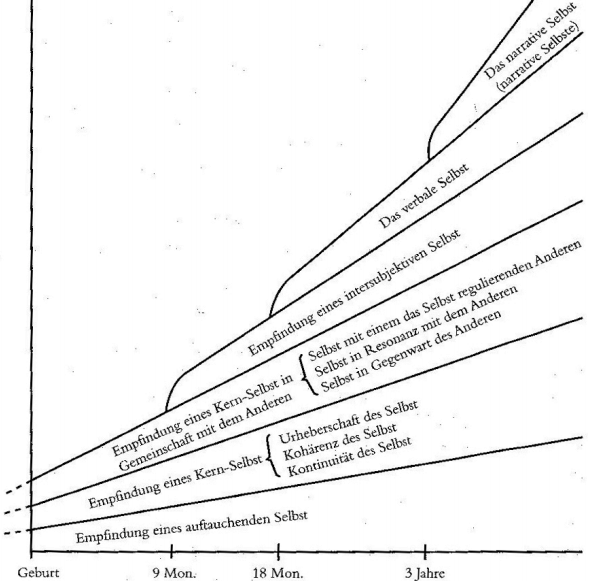
\includegraphics[width=0.7\textwidth]{selbstempfindungen}
  \caption{Die sechs Selbstempfindungen nach Daniel Stern}
  \label{fig:selbstempfindungen}
\end{figure}

Da an dieser Stelle nicht auf alle Bereiche des Selbstempfindens ausführlich eingegangen werden kann, empfiehlt sich ein Blick in Daniel Sterns Werk "Die Lebenserfahrung des Säuglings", in welchem der Entwicklungspsychologe, Säuglingsforscher und Psychoanalytiker in sehr anschaulicher Weise die Entwicklung des Säuglings anhand der Entwicklung eines umfassenden Selbstempfindens erläutert.

In Bezug auf eine entwickelte COPD scheint es naheliegend, sich mit der Entwicklung eines Kern-Selbst und hier insbesondere mit der Invarianz der Urheberschaft zu beschäftigen, wobei nicht außer Acht gelassen werden darf, dass alle Bereiche ineinander greifen und sie letztlich nur theoretisch auseinanderdividiert werden können.

Nun aber warum scheint eine besondere Auseinandersetzung mit der o.g. Invarianz in Bezug auf eine COPD sinnvoll?!

Das Empfinden eines Kern-Selbst entsteht aus dem Zusammenspiel der zuvor genannten Invarianzen der Selbsterfahrung, d.h. unveränderlicher Erfahrungsmuster, die zu einer Organisation und Struktur innerer Prozesse führen. Wie aus der Grafik hervorgeht, handelt es sich um Entwicklungsbereiche, die sich hier natürlich auf den Lebensanfang beziehen, jedoch die Grundlage jeglicher Selbstempfindung bilden. So können sich die einzelnen Bereiche immer weiter ausdifferenzieren, die Basis jedoch bleibt bestehen. 
Stern beschreibt das "Kern-Selbst-Empfinden […] (als) ein erfahrungsgeleitetes Empfinden von Vorgängen, das wir normalerweise als völlig selbstverständlich voraussetzen und uns nicht bewusst machen. […] Das Selbstempfinden ist kein kognitives Konstrukt; es ist die Integration des Erlebens.“ \autocite[106f.]{stern2007} Er bezeichnet es sogar als "die Grundlage für alle differenzierten Selbstempfindungen, die sich später entwickeln werden“ \autocite[106f.]{stern2007}. 

Was passiert jedoch, wenn ein Mensch spürt, dass er zuvor selbstverständliche körperliche Prozesse, wie im Fall der COPD die Atmung, nicht mehr so steuern kann, wie er möchte? Dies spricht m.E. in erster Linie die Invarianz der Urheberschaft an. Sie umfasst das Empfinden, Urheber eigener Handlungen zu sein als auch Nicht-Urheber der Handlungen anderer. Dies ist stets verbunden mit einem willentlichen Vorgehen, der propriozeptiven Wahrnehmung als auch dem Wissen, dass dieses Vorgehen bestimmte Konsequenzen nach sich zieht \autocite[vgl.][106, 114f.]{stern2007}. Im Falle der pneumologischen Veränderungen bei einer COPD, welche stets einhergehen mit ansteigender Atemnot scheint dieses Gefüge nun ins Wanken zu kommen: die Atmung als "selbstverständlicher" und meist nicht bewusst gesteuerter Vorgang verändert sich und dem COPD-Patienten scheint die Kontrolle über diesen Vorgang in manchen Situationen zu entgleiten. Dabei gerät jedoch primär der erste Teil dieser Invarianz, das willentliche Vorgehen, in eine unsichere Position, während die propriozeptive und im Falle der COPD auch die viszerozeptive Wahrnehmung intakt ist und eine Konsequenz für diese körperlichen Vorgänge erahnt werden kann. Dies kann verständlicherweise zu Unsicherheit führen. Bei Menschen, die über ein stark ausgebildetes Ich, ein haltendes und unterstützendes soziales Umfeld sowie über ausreichende Copingstrategien verfügen, wird der Bedarf an professioneller therapeutischer Begleitung vermutlich nicht so hoch sein, wie bei oben beschriebenem Klientel, welches aufgrund einer frühen mangelnden bzw. adäquaten Zuwendung nicht über die genannten Ressourcen verfügen. 

Wiederholt sich dieser Vorgang stetig, kann es zu einer Schwächung regulierender Selbstobjekte führen, welche bereits im Säuglingsalter durch die Interaktion mit einem selbstregulierenden Anderen beginnen, sich herauszubilden \autocite[vgl.][338f.]{stern2007}. Je nach individueller Ausprägung der regulierenden Selbstobjekte kann dieser Vorgang früher oder später in eine Regression des Patienten münden. Nun wird die Regulierung auftauchender affektiver Zustände im Außen wieder wichtiger. 
An dieser Stelle kann an eine frühe Erfahrungswelt im Rahmen eines therapeutischen Settings angeknüpft werden, wenn ein geschützter, haltender, stützender und/oder nährender Rahmen geschaffen werden kann \autocite[vgl.][58ff.]{timmermann2008}. Insbesondere die Arbeit mit der Stimme eignet sich hier besonders. Da die Stimme der primären Bezugspersonen am Anfang des Lebens i.d.R. verbunden wird mit der Erfahrung eines geschützten, nährenden Raums, "werden wir [lebenslang] in den Tiefen unseres Unbewussten mit Stimmausdruck eine >heile Welt< assoziieren" \autocite[282]{deckervoigt2000}. Das "heil" bezieht Decker-Voigt in diesem Zusammenhang darauf, dass uns der Klang der Stimme an eine Zeit erinnere, in der wir Kränkungen, Beängstigungen und Verletzungen seelisch noch ertragen konnten \autocite[vgl.][282]{deckervoigt2000}. 

Darüber hinaus scheint in Bezug auf eine angstfreie Ausbildung eines Kern-Selbst auch ein sicherer, haltender Rahmen notwendig. Greift man zurück auf die Erfahrungen des Säuglings, so wissen wir, dass die Entwicklung stets gekoppelt ist an die Verfügbarkeit der primären Bezugspersonen und ihrem Umgang mit dem Säugling. Für eine gelingende Entwicklung ist es wichtig, dass die primären Bezugspersonen (i.d.R. Mutter und Vater) feinfühlig auf das Kind eingehen und als sichere emotionale Basis für das Kind verfügbar sind (Begriffe aus der Bindungstheorie nach J. Bowlby und M. Ainsworth, siehe \cite{brisch2013}) sowie durch Synchronisationsprozesse mit dem Säugling zur Ausbildung einer stabilen psychischen Struktur beitragen. Da zu Beginn des Lebens noch nicht die Möglichkeit zur Selbstregulation gegeben ist, sind auch für diesen Funktionsbereich die primären Bezugspersonen von großer Wichtigkeit. Wird der Säugling allein gelassen mit dieser Überstimulierung durch unbekannte Reize und kann sein eigenes Gefühlschaos nicht selbst regulieren, wird er sich vermutlich ängstlich zurückziehen. Hat er jedoch im Außen ein (markiert) spiegelndes \autocite[vgl.][153]{fonagy2004}, feinfühliges Gegenüber, so kann er nach und nach diese nun sich ausbildenden Repräsentanzen in seine psychische Struktur integrieren. 
Übertragen auf die Situation eines erwachsenen Menschen mit COPD kann dies bedeuten, dass er für die Bewältigung seiner gesundheitlichen Krise und zur Prävention vor komorbiden psychischen Störungen von einem regulierenden Anderen profitieren würde. Häufig jedoch sind die näheren Angehörigen aufgrund eigener Involviertheit nicht in der Lage, diesen stützenden Part zu übernehmen oder die Beziehung ist aufgrund der Krankheitssituation bereits zu sehr belastet. 

Daher kann es hilfreich sein, außerhalb der gewohnten sozialen Bezüge einen Raum für sich in Anspruch nehmen zu können, in dem es um die eigene Person geht, so wie sich zu Beginn des Lebens in einem geschützten Rahmen die Handlungen der Bezugspersonen am Säugling orientieren. Im Rahmen einer tiefenpsychologisch fundierten Musiktherapie, wie sie in dieser Arbeit vertreten wird, steht stets der "Musik erlebende und sich durch Musik ausdrückende Mensch als Klient" im "Zentrum der Aufmerksamkeit" \autocite[4]{timmermann2004}. Für den Umgang mit der Erkrankung bringt jeder vor dem Hintergrund seiner individuellen Kindheitsgeschichte Copingstrategien und Ressourcen mit, die ihm helfen, die Situation, zu bewerkstelligen. In manchen Fällen ist es jedoch sinnvoll, sich dieser gewahr zu werden, zu verstehen, wie und aus welcher Situation diese entstanden sind und neue Wege auszuprobieren. 

\section{Therapeutische Grundhaltung} 
Wie im vorherigen Kapitel ersichtlich, bildet das psychoanalytisch-tiefenpsychologische Verständnis von seelischen Prozessen sowie entwicklungspsychologisches Wissen die Grundlage meiner Arbeit. Meine Grundhaltung ist jedoch mit den Jahren durch die Auseinandersetzung mit anderen Schulen (u.a. während meines Sozialpädagogikstudiums) gewachsen und beinhaltet daher Schulen-übergreifende Aspekte. 

Für die therapeutische Arbeit erachte ich den Aufbau einer haltenden, vertrauensvollen Beziehung, welche von Respekt und Achtsamkeit geprägt ist, als wesentlich. 
Im Rahmen dieser ist es die Aufgabe des Therapeuten, empathisch und kongruent auf sein Gegenüber einzugehen, stets dessen Individualität und subjektive Wahrnehmung akzeptierend. 
Es geht für mich um Begleitungs- und Verstehensprozesse, welche die unterschiedlichen Ebenen der therapeutischen Arbeit, Übungs-, Erlebnis- und Konfliktzentrierung, je nach Kontext und Bedarf nutzt, um darüber hinaus mit dem Patienten angemessene Veränderungs- bzw. Weiterentwicklungsprozesse anzustoßen und voranzubringen. 

In der Arbeit mit COPD-Patienten scheint es m.E. sinnvoll, die Arbeit vorerst primär übungs- und erlebniszentriert sowie ressourcenorientiert auszurichten, da aufgrund begrenzter Zeit (siehe \ref{section:gedanken_zum_setting}) und vermutlicher Abwehr gegenüber einem psychotherapeutischen Verfahren eine tiefere Bearbeitung bestehender Konflikte nicht sinnvoll erscheint insbesondere im Hinblick auf die Erreichung der Therapieziele. Nicht sinnvoll daher, weil ein weiteres Auffangen und Bearbeiten evtl. aufgrund des Settings (siehe \ref{section:gedanken_zum_setting}) nicht mehr möglich ist. Sollte es jedoch im Verlauf der Behandlung sinnvoll oder gar notwendig erscheinen, auf solche tiefer einzugehen, ist dies natürlich nicht ausgeschlossen. Allerdings ist es hier erforderlich, immer wieder zu hinterfragen, ob dies tatsächlich für den Patienten momentan tragbar oder evtl. sogar zu überfordernd ist. Insbesondere dann, wenn dies in der Gegenübertragung spürbar wird. Dieser Aspekt ist m.E. für die gesamte Behandlung wichtig, egal auf welcher Ebene gearbeitet wird. COPD-Betroffene sind meist primär mit ihrer Erkrankung beschäftigt und eine bewusste Aufarbeitung psychischer Konflikte könnte schnell destabilisierend wirken, da bereits der Prozess der Krankheitsbewältigung teilweise sehr kraftraubend wirkt. Zu dieser Einschätzung komme ich durch persönliche Gespräche und Erfahrungsberichte von Betroffenen, welche ich im Verlauf der Auseinandersetzung mit der Arbeit geführt oder gehört/ gelesen habe. 

Eventuell ergibt sich aber im Anschluss an eine rehabilitative Maßnahme eine längerfristige ambulante Therapie, welche wiederum neue Möglichkeiten eröffnet. 

Darüber hinaus scheint mir für die therapeutische Arbeit mit diesem Klientel, wie zuvor erläutert, der Sucht-Aspekt sehr wichtig. Ich vermute, dass sich in der Behandlung dieser Patienten diese Abhängigkeitsthematik auch in der Beziehung zum Therapeuten zeigen kann. So könnten einerseits die unbewussten Wünsche nach Ich-verstärkenden Reaktionen bzw. auch das Gegenteil wie oben beschrieben i.S. der Selbstzerstörung an den Therapeuten herangetragen werden. Hier gilt es in der Gegenübertragung sehr aufmerksam zu sein und diese Tendenzen nicht auszuagieren, sondern vielmehr Interventionen anzubieten, welche die Selbstwirksamkeit des Einzelnen stärken und ihn auf sich zurückführen. Gerade bei Patienten mit einer körperlichen Erkrankung scheint mir hier die Aufmerksamkeitslenkung auf den Körper und die Atmung sehr hilfreich. Ohne gleich zu tief in psychische Themen einzusteigen, werden diese doch unumgänglich mit bearbeitet (siehe \ref{section:einbezug von koerper und atem}). 

\section{Therapieziele}
Hierin kann an die vorherigen Ausführungen gut angeschlossen werden. Eines der mir am wichtigsten erscheinenden Ziele ist die Steigerung der Selbstwirksamkeit. Dieser Gesichtspunkt knüpft sowohl an das Sternsche Thema der Urheberschaft als auch an den unter \ref{psychische_komorbiditaet} beschriebenen Circulus Virtuosus an. Die Erfahrung, das eigene Befinden selbst beeinflussen und verändern zu können, kann im Rahmen musiktherapeutischer Stimmarbeit, wie sie hier konzipiert ist, einen wesentlichen Beitrag zur Förderung eines selbstwirksamen Erlebens bieten. Atemvertiefung, sensibilisierte Körperwahrnehmung, Singen als (evtl. wiederentdeckte) Ausdrucksform, die Einbindung in eine und der Austausch innerhalb einer Gruppe sowie positive Beziehungs- und Selbsterfahrungen im Rahmen der therapeutischen Beziehung sind m.E. weitere Aspekte, welche zur Stärkung dieses Bereiches beitragen können.

Mit Fortschreiten der Erkrankung nimmt in der Regel auch die (subjektive) Lebensqualität Betroffener immer mehr ab. Aus diesem Grund scheint es mir als eine wesentliche Aufgabe, die Steigerung der Lebensqualität auch als Ziel in dieses Konzept aufzunehmen. Ein wichtiges Ergebnis neuerer Singforschung, welche sich dem Thema "Singen und COPD" widmete (siehe \ref{copd_in_der_singforschung}, zeigte zudem, dass insbesondere die Lebensqualität Betroffener durch eine regelmäßige Teilnahme an einem Singangebot signifikant gesteigert werden konnte. 

Zudem konnte festgestellt werden, dass durch die Steigerung der Lebensqualität eine geringere Wahrscheinlichkeit zur pathologischen Ausbildung einer depressiven oder Angstsymptomatik bestand, was zudem einen Ausweg aus dem beschriebenen COPD-Teufelskreis bedeuten könnte. So enthält dieses Konzept auch die Absicht der Prävention bzgl. der sich oftmals im Verlauf der COPD zeigenden Komorbiditäten wie Depression und Angst.

Für einige mag gerade die akute Gesundheitsverschlechterung zum ersten als auch zum wiederholten Male zu einem krisenhaften Erleben der eigenen Situation führen. Dies kann durchaus auch mit der Auseinandersetzung der Begrenztheit des eigenen Lebens sowie mit dem bewussten Auftauchen der Todesangst einhergehen. Hier kann es das Ziel musiktherapeutischer Arbeit sein, Patienten einen Ort für die Wahrnehmung, Akzeptanz und den Umgang mit den damit verbundenen Affekten zu eröffnen und sie darin zu begleiten, die Möglichkeiten zum persönlichen Wachstum und zur Weiterentwicklung zu erkennen und zu nutzen, welche jeder Krise innewohnen. Dabei scheint es förderlich, durch den Austausch mit einem oder mehreren Spiel- und Gesprächspartnern und die bewusste Auseinandersetzung mit der bisherigen Selbsteinschätzung und Lebenssituation neue Sichtweisen auf sich und die eigene Lebensbehandlung zu entwickeln. Hier stellt die Musik und insbesondere der stimmliche Ausdruck eine wichtige Ergänzung zur Sprache dar, denn durch den Wechsel vom Darüber-Reden zum Es-Spielen kann ein sehr hilfreicher Ausweg aus den herkömmlichen Denk- und Fühlschablonen geschaffen werden. Hierin enthalten ist zudem das Thema der Krankheitsbewältigung, welches mir für die Arbeit mit diesem Klientel als sehr wesentlich erscheint. Aufgrund der mangelnden psychologischen Betreuung, häufiger sozialer Isolation mit Fortschreiten der Erkrankung sowie seltenem Kontakt zu anderen COPD-Patienten fehlen Betroffenen oftmals Austauschmöglichkeiten über krankheitsimmanente Themen und Fragen und verbleiben so in ihrer eigenen Gedanken- und Phantasiewelt. Hierfür scheint mir die Arbeit in der Gruppe sehr sinnvoll, wie im folgenden Kapitel näher erläutert werden soll.

\section{Gedanken zum Setting}
\label{section:gedanken_zum_setting}
Die vorangegangene Darstellung der therapeutischen Ziele deutet bereits darauf hin, dass in diesem Kontext die Arbeit in der Gruppe sinnvoll erscheint. Insbesondere Patienten, die von sozialer Isolation bedroht sind und Schwierigkeiten (entwickelt) haben, sich in sozialen Gruppen zu bewegen, können in einem geschützten und durch die Therapeutin gehaltenen Rahmen neue Erfahrungen sammeln, diese reflektieren und über diesen Prozess wieder Vertrauen in die eigenen Kontaktmöglichkeiten fassen.

Zudem kann es im Austausch mit der Gruppe zur Hinterfragung der eigenen Lebens-be-handlung kommen und alternative Umgangsformen und Lösungsstrategien entwickelt werden. 

Vielen Patienten fehlt oftmals der Kontakt zu anderen Betroffenen und es fällt ihnen schwer, aus eigenem Antrieb sich an Selbsthilfegruppen oder Beratungsstellen zu wenden. Dies kann auch aus einem geschwächten Gefühl für eigene Bedürfnisse und einer verzerrten Selbstwahrnehmung resultieren. Auch hier kann der Einzelne gerade von der Gruppensituation profitieren, da hier ein Raum für den Abgleich von Selbst- und Fremdwahrnehmung geschaffen werden kann.

Gerade für die Krankheitsbewältigung kann der Austausch innerhalb einer diagnosespezifischen Gruppe daher hilfreich und unterstützend wirken. Um jedoch den oben entwickelten Gedanken in Bezug auf ein haltendes, stützendes und spiegelndes Gegenüber innerhalb eines geschützten Rahmens, in welchem ein Raum zum Ausprobieren, Reflexion, Stärkung und Veränderung geboten wird, gerecht zu werden, bedarf es einer therapeutisch ausgebildeten Leitung dieser Gruppe. 

Zudem scheint mir das Gruppensetting hinsichtlich der Suchtthematik als sinnvoll. Während in der Einzeltherapie die Ablösungsschritte vom Therapeuten zugunsten einer größeren Autonomie beschwerlicher sind, können diese durch die Sicherheit-gebende Gruppe leichter ausprobiert und gegangen werden \autocite[vgl.]{nawe2014}. Gerade in Bezug auf die Stärkung der Selbstwirksamkeit ist dies meines Erachtens ein wichtiger Aspekt.

Um diesen geschützten Rahmen aufrechterhalten zu können und gruppendynamische Prozesse für den Therapeuten überschaubar bleiben, ist eine Gruppengröße von 6-8 Patienten optimal todo Weber. Um Überforderungstendenzen sowohl auf körperlicher als auch auf geistig-seelischer Ebene entgegenzuwirken, wird eine Sitzungsdauer von 50-60 Minuten angestrebt. Zudem ist eine halboffene Gruppenform angedacht, um einerseits den Gruppenprozess nicht allzu häufig zu stören und so evtl. in die Stagnation zu treiben und andererseits möglichst vielen potentiellen Patienten den Zugang zu diesem gruppentherapeutischen Angebot zu ermöglichen. 

Während der Auseinandersetzung mit diesem Masterarbeitsthema entstanden unterschiedliche Ideen, in welchem Rahmen eine Durchführung dieses Konzepts möglich erscheint.
Die erste Idee bestand darin, Betroffene über Selbsthilfegruppen, Arztpraxen und Kliniken zu erreichen und ein ambulantes Angebot zu gestalten. Dies würde jedoch bedeuten, dass Patienten evtl. einen längeren Weg auf sich nehmen müssten, dies jedoch zum Teil aufgrund ihres Gesundheitszustandes nicht bewerkstelligen können. Da  jedoch m.E. regelmäßige Sitzungen mind. 1-2mal wöchentlich gerade für den Anfang sinnvoll erscheinen, um mit einer Gruppe i.S. eines gruppentherapeutischen Konzepts arbeiten und die Erreichung der Ziele realistisch gestalten zu können, ist dieses Setting gerade für den Anfang nicht sinnvoll. Zudem konnte bei einer Kontaktaufnahme mit einer Selbsthilfegruppe viel Widerstand hinsichtlich eines solchen Angebots wahrgenommen werden, was zum einen aus der Sorge resultierte, dass Singen für viele zu anstrengend sei - ich vermute hier jedoch auch einen Zusammenhang mit dem Thema Scham - und zum anderen eine Distanzierung hinsichtlich psychotherapeutischer Begleitung, da sie sich primär auf körperlicher Ebene Unterstützung wünschen. Eine Kollegin berichtete zudem ähnliche Erfahrungen mit dieser Patientengruppe. 
Daher denke ich, dass dieses Konzept am besten eingebettet wäre in ein Setting, welches musiktherapeutische Stimmarbeit als einen Teil der Behandlung ansähe und sie in die Behandlungspläne der Patienten mit aufnähme. Hier sollte der Zugang so leicht wie möglich gestaltet sein, so dass Patienten keine langen extra Wege zu den Sitzungen unternehmen müssen, sondern am besten bereits vor Ort sind. Ein Rahmen, in welchem Patienten über mehrere Wochen in eine fortlaufende tägliche Behandlung eingebunden sind, stellt hierbei die pneumologische Rehabilitation dar. Wie bereits unter \ref{nicht-medikamentoese_therapien} erläutert, kann diese ambulant, teilstationär oder stationär durchgeführt werden. Die psychotherapeutische Begleitung hat hier jedoch nach wie vor einen sehr geringen Stellenwert, lediglich die Raucherentwöhnungsprogramme werden über den Zeitraum der Reha i.d.R. von einem Psychologen durchgeführt. Gespräche mit einem Psychologen sind meist fakultative Angebote. Ansonsten gehören edukative Vorträge zu einer regulären pneumologischen Reha dazu, was sicherlich einen großen Stellenwert hinsichtlich der Krankheitsbewältigung hat, jedoch nicht den Einzelnen mit seinen individuellen Unterstützungsbedürfnissen beachtet. 

Aus Beobachtungen während eigener pneumologischer Rehabilitationsmaßnahmen weiß ich, dass sich trotz vorheriger Skepsis die meisten Patienten zusätzlichen Angeboten wie Ergo- oder Kunsttherapie durch das Ausprobieren öffnen konnten und es ihren Aufenthalt bereicherte. So könnte ich mir auch bei diesem Konzept vorstellen, dass durch eine selbstverständliche Einbettung dieses Angebots in die Behandlung eine größere Akzeptanz und die Bereitwilligkeit, es auszuprobieren, steigen könnte im Vergleich zur ambulanten Arbeit ohne Anschluss an eine solche Institution. 

In Bezug auf den Gedanken eines halboffenen Gruppenangebots (siehe oben) wäre m.E. eine Aufnahme in die Musiktherapie-Gruppe alle 2 Wochen sinnvoll, um zu vielen Wechseln entgegenzuwirken und so eine dem Kontext mögliche Kontinuität zu schaffen. In der Regel finden Neuaufnahmen in der pneumologischen Rehabilitation 2-3mal am Anfang der Woche statt, so dass die ersten Therapien Mitte/ Ende der Woche beginnen können. Wenn möglich wären aufgrund der geringen Teilnehmerzahl zwei parrallel laufende, jedoch versetzt aufnehmende Gruppen, optimal, um Patienten eine Teilnahme über den gesamten Verlauf ihrer Rehabilitationsmaßnahme zu ermöglichen.

Die Anbindung an ein Krankenhaus wurde ebenfalls angedacht, jedoch scheint es auch hier schwierig, eine Kontinuität aufrecht zu erhalten. Aufgrund meist kürzerer begrenzter Aufenthalte könnten hier Singangebote, Einzeltherapien oder musiktherapeutische Kurzinterventionen angedacht werden. Im Sinne einer Gruppenbehandlung sowie für die angedachte Prozessbegleitung sehe ich eine regelmäßige Teilnahme über mehrere Sitzungen für dieses Konzept aber als wichtig an. 

Eine feste Einbindung in ein rehabilitatives Behandlungskonzept könnte zudem bedeuten, dass ein fester Raum für diese musiktherapeutische Arbeit zur Verfügung stünde und somit der Einbezug von Instrumenten gerade zu Beginn der Behandlung, um die anfänglichen Hemmungen besser auffangen zu können, möglich würde. Im ambulanten Setting scheint die Arbeit mit einem größeren Instrumentarium aus logistischen Gründen eher schwierig, es sei denn, es gäbe Lagermöglichkeiten.

Abschließend ist also festzuhalten, dass gerade bei der ersten praktischen Umsetzung dieses Konzepts, welche den nächsten Schritt bedeuten würde, eine Einbindung in eine Einrichtung der pneumologischen Rehabilitation sinnvoll wäre.

\section{Indikation/ Kontraindikation}
Wie bereits unter \ref{psychische_komorbiditaet} erläutert, manifestieren sich Angst- und Panikstörungen sowie Depression bereits in den frühen Stadien der Erkrankung und nehmen in der Regel mit dem Fortschreiten der Erkrankung nicht zu. Daher gilt es hier sich nicht nach den Schweregraden, sondern nach dem Bedarf an psychotherapeutischer Begleitbehandlung zu orientieren. 

Generell gilt jedoch aufgrund des erhöhten Risikos zur Ausbildung einer psychischen Komorbidität für jeden Patienten, der daran Interesse hat und davon profitieren könnte, eine Möglichkeit zur Teilnahme an diesem therapeutischen Behandlungsangebot bereitzuhalten, da ein wichtiges therapeutisches Ziel in der Prävention zur Ausbildung einer psychischen Erkrankung als auch der Krankheitsbewältigung liegt.

Wie bei jeder gruppentherapeutischen Behandlung gelten auch hier folgende Ausschlusskriterien: akute Psychosen/ hirnorganische Störungen, Schwierigkeiten, einen Leiter zu akzeptieren und/oder interpersonelle Beeinträchtigungen. Darüber hinaus gilt es die Motivation hinsichtlich der Behandlung zu überprüfen. Weitere mögliche Kriterien zur Gestaltung einer Gruppe im psychotherapeutischen Setting können bei Strauß und Mattke gefunden werden \autocite[vgl.][78-88]{mattke2007}.

Eine weitere Kontraindikation könnte fehlende Mobilität bedeuten, da Teilnehmer das Gruppenangebot selbstständig oder mit Hilfe aufsuchen müssen. Aber auch Menschen, die auf einen Rollstuhl oder dauerhafte Sauerstoffgabe angewiesen sind, können an diesem musiktherapeutischen Angebot teilnehmen. An dem anschließend beschriebenen Studienprojekt in Kent haben ebenfalls Personen teilgenommen, welche auf zusätzliche Sauerstoffversorgung angewiesen waren; diese Personen konnten sich dennoch am Angebot beteiligen. Bei gleichzeitigem Bedarf an psychotherapeutischer Begleitung sollte jedoch bei Patienten, die nicht an dem Angebot teilnehmen können, ein therapeutisches Angebot im aufsuchenden Einzelsetting in Betracht gezogen werden.

Sollte es im Vorgespräch mit einem Patienten Anzeichen für eine Traumatisierung geben, gilt es hier abzuwägen, ob eine Gruppenbehandlung im hier angedachten Sinne angemessen erscheint. Oftmals ist es gerade für diese Patientengruppe wichtig, in einem geschützten und sehr strukturierten Rahmen äußere und innere Sicherheit aufzubauen, um sich dann evtl. freieren Formen anzunähern. Da bei diesen Menschen das "Erstarren und Verstummen [...] einen überlebensnotwendigen Schutz darstellen" \autocite[68]{rittner2012} und Musik einen Trigger für Retraumatisierungen darstellen kann, gilt es hier respektvoll und sehr behutsam vorzugehen.

Wenngleich der Einsatz der (Sing-)Stimme insbesondere im Hinblick auf ein bewussteres und verlängertes (Aus-)Atmen m.E. in diesem Bereich sehr sinnvoll erscheint, so ist gleichzeitig auch Vorsicht geboten. Bei Patienten mit COPD kann es zu entzündlichen Vorgängen rund um den Stimmapparat aufgrund der medikamentösen Behandlung und einer geschwächten Immunabwehr kommen. In diesen Fällen ist es notwendig, durch einen Phoniater abklären zu lassen, ob die Stimme der Schonung bedarf oder aber der gezielte und bedachte Einsatz der Stimme zu einer Besserung der Stimmfähigkeit beitragen kann \autocite[vgl.][103ff.]{alavi2009}.

\section{COPD in der Singforschung}
\label{copd_in_der_singforschung}
In der neueren Singforschung gibt es mittlerweile einige Ergebnisse, die darauf hinweisen, dass der Einsatz des therapeutischen Singens speziell für COPD-Patienten aus unterschiedlichen Gründen von großem Nutzen sein kann. Es wurden hier sowohl positive Effekte in Bezug auf physische Parameter (wie z.B. Verbesserung der Lungenfunktion) als auch auf psychosoziale Faktoren (wie die Steigerung der Lebensqualität) gemessen.
In der englischsprachig textbasierten Meta-Datenbank Pubmed, welche die weltweit umfassendste Datenbank für medizinische und psychologische Artikel darstellt, konnten zum Thema Singen und COPD/Lungenemphysem insgesamt sieben relevante Studien sowie eine aktuelle Literaturrecherche gefunden werden \autocite{pmid19436683,pmid20175359,pmid20682030,pmid23145504,pmid23497924,pmid23497929,pmid24398814,pmid24793633}. Die Ergebnisse sind sehr weit gestreut und lassen keine klaren Aussagen über die Wirksamkeit des Singens auf die physische, funktionale oder psychische Konstitution von COPD-Patienten zu. Dies könnte u.a. dem Umstand geschuldet sein, dass die Studiendesigns noch optimiert werden müssten (zu kleine Teilnehmer-Kohorte, zu kurze Studiendauer, wenige randomisierte und kontrollierte Studien). Jedoch kann aufgrund der in unterschiedlicher Ausprägung primär positiven Effekte davon ausgegangen werden, dass COPD-Patienten von therapeutischem Singen, welches auf diese Patientengruppe hinsichtlich der Übungs- und Liedauswahl abgestimmt ist, profitieren könnten.

Die umfangreichste und bisher am größten angelegte Studie, welche jedoch merkwürdigerweise nicht in pubmed auffindbar war, wurde im Zeitraum zwischen September 2011 und Juni 2012 in der traditionellen Grafschaft Kent im Südosten Englands durchgeführt, da in dieser Region die COPD-Prävalenz besonders hoch sei \autocite[vgl.][4]{clift2013}. Der Titel der Studie lautete: "A feasibility study on the health benefits of a participative community singing programme for older people with COPD" \footnote{Eine Videozusammenfassung der Studie kann unter folgendem Link angeschaut werden: https://www.youtube.com/watch?v=c0UK2X3i-FU}.

Im vergangenen Jahr hatte ich die Möglichkeit, den Hauptinitiator dieser Studie, Steven Clift, bei einem Kongress der Singenden Krankenhäusern zu erleben und die neuesten Ergebnisse zu diesem Thema aus erster Hand zu erfahren. 

Es handelt sich hierbei um eine relativ groß angelegte Feasibility (Machbarkeits-) Studie (n=109,Durchschnittsalter: 69), jedoch ist das Studiendesign nicht-kontrolliert sowie -randomisiert. Dies entstand aus dem Wunsch heraus, eine Kohorte zu bilden, die die Motivation mitbringt, an einem Singprogramm über 10 Monate lang teilzunehmen, so dass möglichst viele am Ende hinsichtlich der Studienziele überprüft werden können. Dieses Studiendesign sei wichtig als Basis, um daran eine größere randomisierte und kontrollierte Studie anschließen zu können. Die Rekrutierung fand über allgemeinmedizinische Praxen, Community Health-Zentren, Zeitungsausschreibungen und die Britische Lungenstiftung in Kent statt. Die Patienten wurden in insgesamt sechs Gruppen aufgeteilt, welche sich vor Ort einmal wöchentlich über 10 Monate zum professionell angeleiteten Singen trafen (aufgrund einer Weihnachts- und Osterpause insgesamt 30 Sitzungen). Diese Einheiten gingen über 90 Minuten, worin jedoch mind. 30 Minuten Atem-, Körper- und Stimmübungen enthalten waren. Die Patienten brachten in der Regel keine regelmäßigen Singerfahrungen mit.

Ziel war es, herauszufinden, von welchen Effekten ältere Menschen mit COPD hinsichtlich der Messwerte Atmung, gesundheitsbezogene Lebensqualität sowie der physischen und psychischen Gesundheit durch ein wöchentliches Singangebot in der Gruppe über einen Zeitraum von zehn Monaten profitieren würden. 

Die Teilnehmer wurden am Anfang, in der Mitte (nach 5 Monaten) und am Ende beurteilt und mussten zu diesen Zeiten ebenfalls sowohl einen Fragebogen zum Thema Lebensqualität (St. George's Respiratory Questionnare, SGRQ) als auch einen zum Thema "Nutzung des Gesundheitssystems" ausfüllen. Die Lungenfunktionstestung wurde am Anfang und am Ende durchgeführt. 

Die Studienergebnisse zeigen zum Einen eine signifikante (p=0,006) Verbesserung der Lungenkapazität (Steigerung des FEV1 um 2\% nach 10 Monaten) und zum Anderen eine Steigerung der Lebensqualität um 3 Messpunkte. Dieser Wert ist der Beste, der jemals mithilfe medikamentöser Behandlung bei COPD-Patienten erzielt werden konnte \autocite[vgl.]{clift2013a}. So berichteten Teilnehmer, dass sich die regelmäßige Teilnahme an der Singgruppe sehr positiv auf ihr soziales Leben sowie ihre physische und psychische Konstitution ausgewirkt hätten \autocite[vgl.][6ff.]{clift2013}

\section{Einbezug von Körper und Atem} 
\label{section:einbezug von koerper und atem}
Atemvertiefung
Massage der Bauchorgane
Beweglichkeit des Brustkorbs und Lockerung der Atemhilfsmuskulatur
Verbesserung der Beweglichkeit des Zwerchfells
Durch Atemvertiefung entstehen Momente des Loslassens, der Entspannung. In dieser Entspannung können nun auch durch den zuvor bestehenden Stress überlagerte Gefühle hervortreten und Raum bekommen. 
Verbindung Emotionales Erleben und Atmung/ Körper




%Da es sich bei der COPD primär um eine körperliche Erkrankung handelt, soll an dieser Stelle noch eine weitere Theorie, die des "Embodiments", hinzugezogen werden, die sich auf die Wechselwirkung von Körper und Psyche bezieht. 

%Vier Vertreter unterschiedlicher Disziplinen (Kognitionswissenschaften, Psychologie, Neurobiologie und Körperarbeit) haben zusammengetragen, was aus ihren unterschiedlichen Blickwinkeln zum Zusammenhang von Körper und Psyche wichtig erscheint. Entstanden ist diese Zusammenarbeit aus der gemeinsamen Erfahrung, dass der Zusammenhang von Psyche und Körper in vielen Bereichen noch mangelhaft Beachtung findet und gerade in therapeutischen und beratenden, aber auch wissenschaftlichen Arbeitsfeldern, in deren Fokus der Mensch steht, wichtiger Bestandteil der Betrachtung des Einzelnen sein sollte.
%Storch, Cantieni, Hüther und Tschacher haben jedoch in ihrer Publikation nicht das Rad neu erfunden, sondern bestehendes Wissen und Ideen zum Thema zusammengetragen und weiterentwickelt. Embodiment-Theorien gehen davon aus, dass eine Wechselwirkung "zwischen allem, was als Körpergeschehen aufgefasst werden kann (dies beinhaltet einzelne motorische Aktionen und Bewegungsabläufe bis hin zu ganzen Verhaltenssequenzen) und dem psychischen System" \autocite[39]{hüther2010} besteht. todo

%Körper- und Atemwahrnehmung sind jedoch nicht nur zur Unterstützung der Atemwegserkrankung sinnvoll und wichtig, sondern auch Achtsamkeit in Bezug auf die Sucht im Hier und Jetzt sein -> MBSR.

Schlaffhorst Andersen
MT und Atem (Buch)
Annette Cramer
Rittner
Hertha Richter

\section{Praktische Umsetzung}
In einem geschützten Raum wird die Möglichkeit geschaffen, in Kontakt zu gehen, sich auszutauschen eigenes Erleben zu teilen und zu reflektieren. In der Gruppe Rückhalt zu finden, sich nicht mehr isoliert und alleine mit der Erkrankung zu fühlen, dies jedoch in einem therapeutischen Rahmen, welcher die Chance für die Hinterfragung der eigenen Lebensbehandlung sowie zur Veränderung bietet, sind die Intention dieses Konzepts. Abgestimmt auf das Krankheitsbild soll jedoch nicht nur auf der kognitiven, Gesprächsebene angesetzt werden, sondern über Körper- und Atemübungen bis hin zum stimmlichen Ausdruck die eigene Körpersensibilität und der Zugang zur eigenen emotionalen Verfassung und ihrem Ausdruck ausgeweitet werden, um dadurch wieder zu mehr Sicherheit und Selbstvertrauen in die eigenen selbstwirksamen Kräfte zu gelangen. Wenn die institutionellen und finanziellen Rahmenbedingung es ermöglichen, wäre ein Grundinstrumentarium hilfreich, insbesondere in der Anfangsphase, jedoch nicht notwendig. Der Einstieg über die instrumentale Improvisation kann hinweghelfen über die Hemmung des Stimmeinsatzes (wie weiter zuvor bereits erläutert).  

%Nachdem unter \ref{psychodynamische ueberlegungen} einige psychodynamische Phänomene bei einer Suchtproblematik zusammengetragen wurden, sollen diese nun auch bei den Überlegungen zum Aufbau und Inhalt der Sitzungen Berücksichtigung finden. 

In Bezug auf das Thema "Scham" sowie auf möglicherweise auftretende Widerstände gegenüber dem Singen sollten die Stunden zu Beginn sehr klar strukturiert werden; sowohl vom Aufbau als auch im musikalischen Tun. So stehen am Anfang Körper- und Atemwahrnehmung im Vordergrund. Darauf aufbauend scheint es mir sinnvoll, evtl. mit Rhythmusinstrumenten, dem Körper, Atem und/ oder Stimme rhythmische Übungen einzuführen, um Sicherheit in diesem Kontext aufzubauen. Der stimmliche Ausdruck kann vorsichtig im Rahmen von Atemübungen angebahnt werden. So bietet sich hier beispielsweise die Vokalraumarbeit nach Ilse Middendorf an, bei welcher Vokale vor dem Erklingen imaginiert werden. Bevor die Vokale erklingen, werden sie geatmet, indem die Formung des Vokals primär im Ansatzrohr simuliert, jedoch nicht an den Stimmlippen in Schwingung versetzt und dadurch hörbar wird. Erst wenn der Vokal dem Übenden klar geformt erscheint, wird er langsam vernehmbar. Interessant ist dabei, dass ohne das Ertönen-Lassen der Atem bereits in verschiedene Bereiche fließt je nach Wahl eines Vokals oder aber auch Konsonanten. Bei Middendorf gibt es hierzu schematische Aufzeichnungen \autocite[vgl.][60ff.]{middendorf1995}. Diese Übungen sind sehr gut geeignet, um die eigenen Atemräume besser zu erkunden und gleichzeitig in einem leistungsfreien Raum das Ertönen-Lassen der eigenen Stimme auszutesten. 

Hilfreich ist für den Aufbau eines Sicherheit und Halt gebenden Rahmens zudem das Einführen von Ritualen. Das Ritual als sicheres Kontinuum stellt m.E. gerade bei Menschen mit COPD  einen wichtigen Aspekt vor dem Hintergrund plötzlich auftretender Atemnot und Krankheitsverschlechterung dar. Dies soll sich im Folgenden sowohl in der Struktur des möglichen Sitzungsaufbaus als auch in einzelnen Gesten in der späteren praktischen Umsetzung wiederspiegeln.

Im Verlauf der Auseinandersetzung mit diesem Masterarbeitsthema wurden in Fort- und Weiterbildungen (Singende Krankenhäuser, ein atemtherapeutisches Seminar bei Matthias Grot, Wochenendseminare bei Astrid Schmid zur Methode "Atem-Tonus-Ton") sowie Selbsterfahrungsseminaren etliche Übungen und Ideen gesammelt. Da die schriftliche Ausführung dieser Sammlung jedoch den Rahmen dieser Arbeit sprengen würde, wurde dem Anhang eine Liste mit möglicher Literatur insbesondere für den praktischen Teil beigefügt.

\subsection{Überlegungen zum Aufbau der Sitzungen}
Symbolisierung: Geben und nehmen stein, sich verbinden

mit kleinen Einheiten beginnen, um Abwehr zu reduzieren sicherheit Struktur. evtl mit summen einsteigen, feine Vibration, ich bin da, hörbar, aber zeig noch nicht so viel von mir

Ressourcenorientiert und auf die Bedürfnisse der Patienten abgestimmt wird die Stunde gestaltet.

Vom Strukturierten zu immer Freieren Stimmäußerungen
Mischung aus Atem- Körperwahrnehmung, Tönen, Liedern, Stimmimprovisationen evtl. unter Hinzunahme anderer Instrumente…(wäre sicherlich für bestimmte Situationen hilfreich, jedoch nicht in jedem Rahmen umsetzbar). 
Aufmerksamkeitslenkung. 

Ankommen: 
Begrüßung, Frage in die Runde, wie jeder einzelne heute hier ist, ob er ein bestimmtes Thema mitgebracht hat, ihn etwas bewegt, was er teilen möchte etc. evtl. herausarbeiten eines gemeinsamen Themas, worüber zu einem späteren Zeitpunkt improvisiert werden, in einer geleiteten Imagination oder einem thematisch passenden Lied dieses aufgegriffen werden kann.

Warming Up: 
Körperwahrnehmung, Atemwahrnehmung, gezielte Atemübung, die eigene Stimme zum Klingen bringen. Dieser Teil ist sehr wichtig, um auf das Singen vorzubereiten. Je besser die Konzentration auf den Ausatem gelenkt und eine entspannte Körperhaltung eingenommen wird, desto leichter und lustvoller wird die spätere Singerfahrung. Wie in der Singforschung gezeigt werden konnte, kann eine bewusstere und geführte Ausatmung der oftmals unter COPD-Patienten vorherrschenden Schnappatmung (siehe \ref{chapter:copd}) entgegenwirken und so die physische Belastung auch nachhaltig verbessern. Beim darauffolgenden Singen wird dies automatisch geübt, da beispielsweise ein Liedtext sich über eine längere melodische Phrase hinwegziehen kann und die musikalische Ausgestaltung das Einatmen an bestimmten Stellen fordert. Diese musikalischen Bögen würden durch ständiges Zwischenatmen unterbrochen, so dass der musikalisch fühlende und hörende Mensch vermutlich mit der Zeit den Ehrgeiz entwickelt, diese Bögen halten zu können. Natürlich soll im Rahmen dieses Singens jeder in seinem Maße Atmen können, nur wie in der neueren Singforschung bereits belegt werden konnte, gleicht sich die Atmung der Mitglieder einer Singgruppe im Verlauf immer mehr an. Was zum einen körperlich einen großen Effekt hinsichtlich einer ruhigeren, entspannteren Atmung als auch sozial ein Gruppengefühl stiftendes Erlebnis darstellen kann.

In Kontakt gehen: 
Interaktive, auflockernde Übungen (Löwe, Bahn etc.), ritualisiertes Anfangslied, Mantren evtl. gewünschte Lieder die Ausdruck für bestimmte Wünsche, Aussagen des Betreffenden, Hoffnungen, Ängste etc. sein können
(Stärkung der Selbstwirksamkeit: Vokalimprovisation, eigene Ideen für die Ausgestaltung wie z.B. Regeln, Aufbau, zusätzliche Instrumente) Dieser Teil sollte sanft eingeführt werden. Nicht gleich zu Beginn, da es oftmals Überwindung kostet und vor allem Erfahrung mit der eigenen Singstimme und somit Sicherheit mit dergleichen bedarf.

Rezeptiv: 
Besungen/ bespielt werden, die Erfahrung des umsorgt Seins ansprechend

Abschluss: 
zurückkehren in die Runde. Austausch der Erfahrungen, entstandener Fragen, des aktuellen Befindens. Ausblick, Evtl. Abschlusslied

%\subsection{Beispiele für Körper-, Atem-, und Stimmübungen sowie methodische Möglichkeiten der Stimmarbeit}

\section{Abschließende Betrachtung}




%: ----------------------- paths to graphics ------------------------
% change according to folder and file names
\ifpdf
    \graphicspath{{5_konzept/figures/PNG/}{5_konzept/figures/PDF/}{5_konzept/figures/}}
\else
    \graphicspath{{5_konzept/figures/EPS/}{5_konzept/figures/}}
\fi

\newpage\thispagestyle{empty}
% ---------------------------------------------------------------------------
%: ----------------------- end of thesis sub-document ------------------------
% ---------------------------------------------------------------------------
